\documentclass{article}

\usepackage{tikz}
\usetikzlibrary{arrows}

\begin{document}

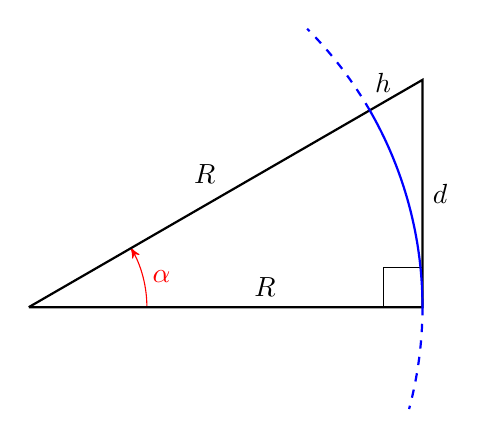
\begin{tikzpicture}
 % angle alpha
 \draw[->,red,>=stealth'] (1.5,0) arc (0:30:1.5);
 \draw[red] (15:1.5) node[right]{$\alpha$};
 % angle droit
 \draw (4.5,0)|-(5,0.5);
 % triangle
 \draw[thick] (0,0)-- node[pos=0.6,above]{$R$} (5,0)
                   -- node[midway,right]{$d$} (5,{5/sqrt(3)})
                   -- node[pos=0.1,above]{$h$}
                      node[pos=0.5,above left]{$R$}(0,0);
 % arcs
 \draw[blue,thick,dashed] (0:5) arc (0:-15: 5);
 \draw[blue,thick] (0:5) arc (0:30: 5);
 \draw[blue,thick,dashed] (30:5) arc (30:45: 5);
\end{tikzpicture}

\end{document}
